\documentclass[a4paper]{report}
%Begin: Thêm các package cần thiết%
\usepackage[utf8]{vietnam} %Gói dùng tiếng Việt%
\usepackage[left=3.5cm,right=2.5cm,top=2cm,bottom=2cm]{geometry}  %Gói canh lề%
\usepackage{draftwatermark} %Gói watermark%
\usepackage{minitoc} %Gói mục lục động %
\usepackage{xurl} 
\usepackage{scrextend}
%Begin: Giao diện mục lục
\usepackage{hyperref}
\hypersetup{
    colorlinks=true,
    linkcolor=blue,
    filecolor=magenta,      
    urlcolor=cyan,
    pdftitle={Overleaf Example},
    pdfpagemode=FullScreen,
    }
\urlstyle{same}
%End: Giao diện mục lục
\usepackage{subfigure}
%End: Thêm các package cần thiết%
\changefontsizes{16pt}
\setlength{\parindent}{0pt}
%Begin: Thêm watermark%
\SetWatermarkAngle{45}
\SetWatermarkColor[gray]{0.97}
\SetWatermarkFontSize{5cm}
\SetWatermarkText{KNNN EZI}
%End: Thêm watermark%

\begin{document}
\begin{titlepage}
%Begin: Bìa%
\begin{center}
    \vspace{5pt}
    \textbf{ĐẠI HỌC QUỐC GIA THÀNH PHỐ HỒ CHÍ MINH}
    \vspace{5pt}
    \textbf{TRƯỜNG ĐẠI HỌC CÔNG NGHỆ THÔNG TIN}
\end{center}

\vspace{5pt}

\begin{center}
    
\includegraphics[scale=0.3]{UIT.jpg}
    \vspace{10pt}
    \fontsize{15pt}{15pt}\selectfont

    \begin{flushleft}
    \fontsize{15pt}{15pt}\selectfont  
    \textbf{\textsl{MÔN HỌC:}~~~~~~{KỸ NĂNG NGHỀ NGHIỆP}}
    \end{flushleft}
\end{center}


\begin{flushleft}
    \fontsize{15pt}{15pt}\selectfont  
    \textbf{\textsl{ĐỀ TÀI:}~~~~~~~~~~{LÀM QUEN VỚI GITHUB}}
\end{flushleft}


\vspace{15pt}
\textbf{GV hướng dẫn: Thái Huy Tân}

\vspace{10pt}
\textbf{Nhóm sinh viên thực hiện:}
\begin{tabbing}
\hspace{9cm}\=\hspace{3cm}\=\ \kill
{\it \textbf{Họ và tên}}\>{\it \textbf{MSSV}}\>\\
\begin{bfseries}Võ Thanh Nhàn\end{bfseries}\> \begin{bfseries}22521009\end{bfseries}\\
\begin{bfseries}Lê Tiến Quyết\end{bfseries}\> \begin{bfseries}21520428\end{bfseries}\\
\begin{bfseries}Nguyễn Viết Đức\end{bfseries}\> \begin{bfseries}22520273\end{bfseries}\\
\begin{bfseries}Huỳnh Nhật Minh\end{bfseries}\> \begin{bfseries}22520862\end{bfseries}\\
\begin{bfseries}Bùi Nhật Phi\end{bfseries}\> \begin{bfseries}22521078\end{bfseries}\\
\end{tabbing}
%End: Bìa%
\vspace{10pt}
\end{titlepage}
\newpage
\tableofcontents
\newpage
\chapter{Giới thiệu về Git, GitHub và giao diện cơ bản}
\section{Giới thiệu về Git}
\textrm{Git là hệ thống kiểm soát mã nguồn mở và miễn phí.}
\newline
\textrm{Git ra đời vào năm 2005 và được phát triển bởi \href{https://vi.wikipedia.org/wiki/Linus_Torvalds}{Linus Torvalds} để hỗ trợ viết Linux kernel.}

\begin{figure}[ht]
    \centering
    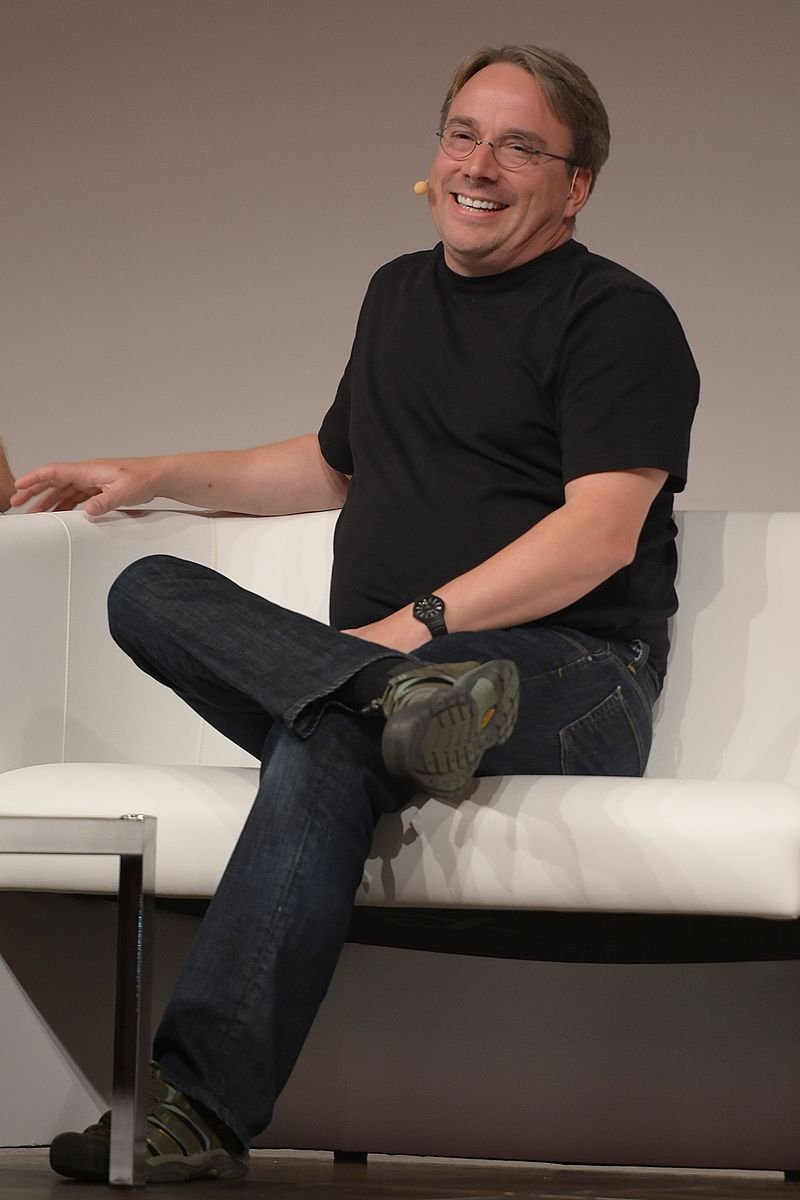
\includegraphics[scale=0.7]{Linus Torvalds.jpg}
    \caption{Hình ảnh của Linus Torvalds}
\end{figure}

\textrm{Toàn bộ code và lịch sử thay đổi dữ liệu sẽ được lưu trữ trên máy người dùng.}
\textrm{Lợi ích khi sử dụng Git:}
\begin{itemize}
    \item \textrm{Dễ sử dụng, thao tác nhanh,gọn, lẹ và rất an toàn.}
    \item \textrm{Giúp quy trình làm việc nhóm đơn giản hơn.}
    \item \textrm{Có thể giúp mọi người làm việc mọi lúc mọi nơi.}
\end{itemize}


\section{Giới thiệu về GitHub}
\textrm{Sự phát triển của nền tảng bắt đầu vào ngày 19 tháng 10 năm 2007. Trang web được đưa ra vào tháng 4 năm 2008 do \href{https://en.wikipedia.org/wiki/Tom_Preston-Werner}{Tom Preston-Werner}, \href{https://en.wikipedia.org/wiki/Chris_Wanstrath}{Chris Wanstrath} và \href{https://en.wikipedia.org/wiki/P._J._Hyett}{PJ Hyett} thực hiện.}
\begin{figure}[ht]
    \centering
    
\includegraphics[scale=0.15]{Github_Dev.jpg}
    \caption{\centering{PJ Hyett, Tom Preston-Werner, Chris Wanstrath \newline (lần lượt từ trái sang phải).}}
\end{figure}
\newline
\textrm{Được xem như mạng xã hội của lập trình viên. Giúp mọi người có thể cùng giao tiếp với nhau, cùng nhau thảo luận, cùng nhau làm việc.}
\newline
\textrm{Có 3 khái niệm quan trọng: Repository, Commit và Branch.}

\subsection{Repository}
\textrm{Repository là một kho lưu trữ các files của dự án. Các files đó có thể là: code, hình ảnh, âm thanh ... mọi thứ liên quan đến dự án.}
\newline
\textrm{Hai loại kho lưu trữ trong Github là Local Repository và Remote Repository.}
\begin{itemize}
    \item Local Repository : là một Repository nằm trên máy tính của bạn, có thể đồng bộ hóa với Remote Repository bằng các câu lệnh của git.
    \item Remote Repository : là một Repository được cài đặt trên server chuyên dụng như là GitHub, GitLab ... 
\end{itemize}

\subsection{Commit}
\textrm{Là những hành động thêm/xóa/sửa file hay thư mục vào trong Repository. Repository lúc này sẽ tạo ra commit để ghi lại sự khác biệt từ trạng thái commit lần trước với trạng thái hiện tại.}
\newline
\textrm{Các commit được chứa tại Repository nối tiếp nhau theo thứ tự thời gian.}

\subsection{Branch}
\textrm{Branch được dùng để phân nhánh và ghi luồng của lịch sử.}
\newline
\textrm{Dùng branch để triển khai dự án theo hướng cô lập để không ảnh hưởng đến công việc của những người khác.}
\newline
\textrm{Khi công việc đã hoàn thành, bạn có thể nhập branch của mình vào branch cũng những người khác.}

\section{Giao diện cơ bản}
\begin{figure}[ht]
    \centering
    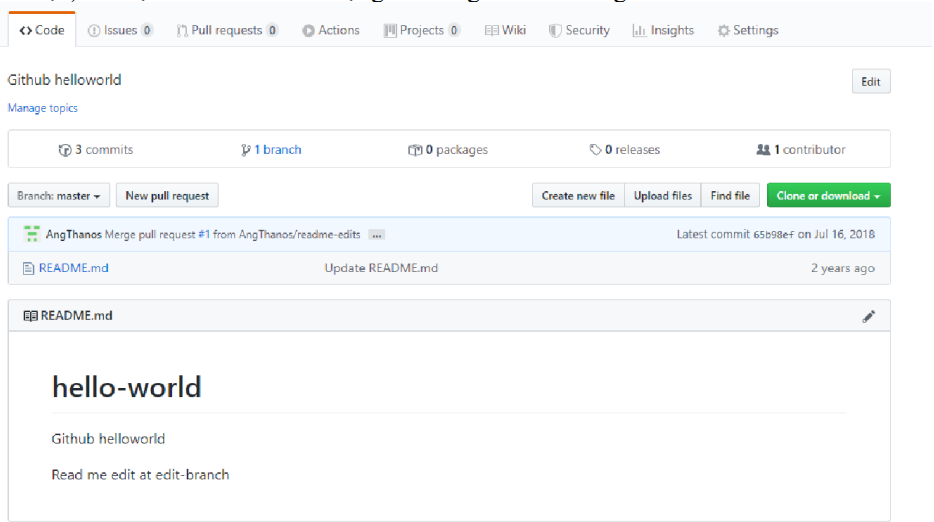
\includegraphics[scale=0.9]{interface_github.png}
    \caption{Giao diện sử dụng của một project}
\end{figure}

\subsection{<> Code}
\textrm{Tổng quan :}
\begin{itemize}
    \item Nơi để xem các tệp và thư mục trong Repository.
    \item Biết được cấu trúc file của dự án.
    \item Xem qua từng file và xem được lịch sử commit.
\end{itemize}
\textrm{Branch :}
\begin{itemize}
    \item Liệt kê tất cả các branch có trong Repository.
    \item Có thể chọn để chuyển giữa các branch với nhau.
\end{itemize}

\subsection{Issues}
\textrm{Tổng quan :}
\begin{itemize}
    \item Nơi để quản lý và theo dõi các task liên quan đến dự án, bug, yêu cầu features.
    \item Các issues có thể được gán nhãn (labels), giao cho từng cá nhân và gắn với pull request.
\end{itemize}
\textrm{Labels : quản lý các nhãn gán dán vào issues.}
\newline
\textrm{Milestone : nhóm các issues lại và có một cách để keep track và kiểm tra quá trình.}
\newline
\textrm{New issues : tạo issues mới (dán nhãn, assign người làm).}

\subsection{Pull request}
\textrm{Tổng quan :}
\begin{itemize}
    \item Tab này được dùng để quản lý và xem các Pull request.
    \item So sánh các branch với nhau.
    \item {Xem được các request đã open và close.}
\end{itemize}
\textrm{Files changed : khi chọn một Pull request để coi, thì mình có thể xem được sự thay đổi mà request này đưa tới thông qua trang này.}
\newline
\textrm{Commit : xem được danh sách cụ thể bao gồm trong request, giúp theo dõi lịch sử thay đổi.}

\subsection{Project}
\textrm{Tổng quan : tab này cho phép tạo ra một project boards để track công việc, sắp xếp task và lên kế hoạch cho các milestone.}

\subsection{Wiki}
\textrm{Tổng quan : là nơi tạo ra và ghi lại doc cho project của mình.}

\subsection{Security}
\textrm{Tổng quan : tab này cung cấp thông tin về bảo mật của Repository bao gồm các lỗ hổng đã biết trong phần phụ thuộc và gợi ý cách khắc phục.}

\subsection{Insight}
\textrm{Tổng quan : cung cấp các phân tích và data liên quan tới Repository. Có thể biết được các thông tin như: code frequency, contributors, ...}

\chapter{Các tập lệnh cơ bản}
\section{git init}
\textrm{Câu lệnh \textbf{git init} dùng để tạo một kho lưu trữ trống và mới.}
\newline
\textrm{Nó tạo một thư mục con có tên là \textbf{.git} và thư mục này chứa tất cả các tập tin cần thiết cho kho chứa.} 

\section{git clone}
\vspace{5pt}
\centerline{\textbf{git clone + `URL`}}
\textrm{Thực hiện câu lệnh \textbf{git clone} để tạo một thư mục mới có tên giống tên của Repository đã tồn tại trên Github, bao gồm tất cả các files, branches và commits vào trong máy.}

\section{git branch}
\textrm{Với cú pháp \textbf{git branch} thì dùng để kiểm tra branch hiện tại mà chúng ta đang thực hiện.}
\newline
\textrm{Để xem tất cả các branch hiện đang có thì ta dùng câu lệnh:}
\newline
\centerline{\textbf{git branch -r}}
\newline
\textrm{Ngoài ra để tạo một branch mới thì chúng ta sử dụng câu lệnh:}
\newline
\centerline{\textbf{git branch + `Name of new branch`}}

\section{git add}
\label{subsec:labelone}
\textrm{Sau khi thay đổi dữ liệu ở các files thì bạn cần cập nhật lại các files lên Staging Area với câu lệnh:}
\newline
\centerline{\textbf{git add .}}

\section{git commit}
\label{subsec:labeltwo}
\textrm{Ngay sau khi thực hiện câu lệnh \textbf{git add .} ở
\ref{subsec:labelone} thì cần sử dụng câu lệnh Commit để lưu lại những thay đổi trong Repo:}
\newline
\centerline{\textbf{git commit -m + `Message about changes`}}

\section{git push}
\label{subsec:labelthree}
\textrm{Khi đã thực hiện câu lệnh Commit ở \ref{subsec:labeltwo} thì thông tin mới chỉ được cập nhật lên Local Repository.}
\newline
\textrm{Để cập nhật lên server thì dùng câu lệnh sau:}
\newline
\centerline{\textbf{git push origin + `Name of branch`}}
\newline
\textrm{Muốn xóa một branch nào đó trên server thì ta có thể dùng:}
\newline
\centerline{\textbf{git push origin --delete + `Name of branch to delete`}}

\section{git remote}
\textrm{Ngoài việc cập nhật lên server như đã nói ở \ref{subsec:labelthree}. Nếu chưa tồn tại remote trên server thì ta cần phải thêm mới một remote trước rồi mới push.}
\newline
\textrm{Các câu lệnh để thực hiện điều đó là:}
\newline
\centerline{\textbf{git remote add origin `Remote URL`}}
\newline
\centerline{\textbf{git push origin `Name of branch`}}

\section{git log}
\textrm{Sử dụng câu lệnh \textbf{git log} sẽ cho chúng ta biết thông tin về \textit{người commit, ngày giờ, message} của những lần commit đó.}

\section{git pull}
\textrm{Sau một khoảng thời gian nào đó, sẽ có những thay đổi dữ liệu các files ở trên server. Để cập nhật những thay đổi đó về branch hiện tại trên máy thì chúng ta cần sử dụng câu lệnh:}
\newline
\centerline{\textbf{git pull origin + `Name of branch`}}

\section{git checkout}
\textrm{Để làm việc trên một nhánh nào đó thì chúng ta cần di chuyển tới nhánh đó với câu lệnh:}
\newline
\centerline{\textbf{git checkout + `Name of branch`}}

\section{git merge}
\textrm{Sau khi cập nhật các file và push lên branch mới. Giả sử bây giờ mình cần ghép các files vào nhánh gốc (\textbf{main}).}
\newline
\textrm{Đầu tiên, chúng ta cần di chuyển tới nhánh gốc với câu lệnh:}
\newline
\centerline{\textbf{git checkout main}}
\newline
\textrm{Sau đó để gộp branch cần gộp vào nhánh gốc thì chúng ta dùng lệnh \textbf{merge}:}
\newline
\centerline{\textbf{git merge + `Name of branch to merge`}}

\chapter{Tổng kết}
\textrm{Trong bài viết này thì nhóm đã giới thiệu về Git, GitHub và một số câu lệnh mà nhóm đã tìm hiểu được. Hy vọng qua bài viết này sẽ giúp các bạn hiểu thêm về Git và cách sử dụng chúng trong công việc sao cho hiệu quả.}

\begin{thebibliography}{2}
\bibitem{doc1}
\href{https://viblo.asia/p/nhung-lenh-git-co-ban-can-nho-V3m5W1OyZO7}{Những lệnh git cơ bản cần nhớ (Nguyen Thi Hang)}

\bibitem{doc2}
\href{https://thachpham.com/tools/hieu-them-ve-commit-va-staging-area-git.html}{[GIT] Tìm hiểu về Commit và Stagging Area (Thạch Phạm)}

\bibitem{doc3}
\href{https://www.nobledesktop.com/learn/git/git-branches}{Git Branches: List, Create, Switch to, Merge, Push, Delete (Noble Desktop)}

\bibitem{doc4}
\href{https://www.youtube.com/watch?v=1JuYQgpbrW0&t=515s}{Từ gà tới pro Git và Github trong 20 phút - Tự học Git siêu tốc (Phạm Huy Hoàng)}

\bibitem{doc5}
\href{https://vi.wikipedia.org/wiki/Git_(ph%E1%BA%A7n_m%E1%BB%81m)}{Git (Wikipedia)}

\bibitem{doc6}
\href{https://vn.got-it.ai/blog/git-commit-la-gi-git-commit-duoc-su-dung-nhu-the-nao}{Git Commit là gì? Git Commit được sử dụng như thế nào? (Got It Vietnam)}

\bibitem{doc7}
\href{https://topdev.vn/blog/git-la-gi/#git-co-loi-ich-gi}{Git là gì? Các lệnh git cơ bản mà mọi lập trình viên nên biết (TopDev)}

\bibitem{doc8}
\href{https://vi.wikipedia.org/wiki/GitHub#:~:text=S%E1%BB%B1%20ph%C3%A1t%20tri%E1%BB%83n%20c%E1%BB%A7a%20n%E1%BB%81n,xem%20nh%C6%B0%20giai%20%C4%91o%E1%BA%A1n%20beta..}{Github (Wikipedia)}

\bibitem{doc9}
\href{https://wiki.tino.org/repository-la-gi/}{Github là gì? Repository là gì? Các thuật ngữ liên quan đến Github (TINO GROUP)}
\end{thebibliography}


\end{document}

